% 1977 年上海卷文科第 5 题：六角螺帽示意图
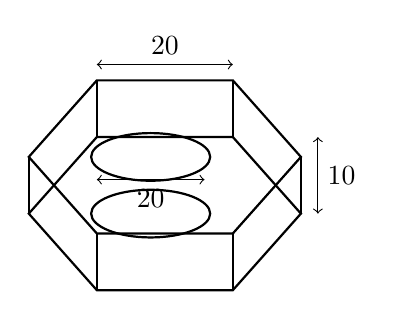
\begin{tikzpicture}[scale=0.72]
  \coordinate (A) at (0,0);
  \coordinate (B) at (2.4,0);
  \coordinate (C) at (3.6,1.35);
  \coordinate (D) at (2.4,2.7);
  \coordinate (E) at (0,2.7);
  \coordinate (F) at (-1.2,1.35);
  \coordinate (A') at (0,-1.0);
  \coordinate (B') at (2.4,-1.0);
  \coordinate (C') at (3.6,0.35);
  \coordinate (D') at (2.4,1.7);
  \coordinate (E') at (0,1.7);
  \coordinate (F') at (-1.2,0.35);
  \draw[thick] (A)--(B)--(C)--(D)--(E)--(F)--cycle;
  \draw[thick] (A')--(B')--(C')--(D')--(E')--(F')--cycle;
  \foreach \p/\q in {A/A',B/B',C/C',D/D',E/E',F/F'}
    \draw[thick] (\p)--(\q);
  \draw[thick] (0.95,1.35) ellipse [x radius=1.05, y radius=0.42];
  \draw[dashed] (0.95,1.35) ellipse [x radius=1.05, y radius=0.42];
  \draw[thick] (0.95,0.35) ellipse [x radius=1.05, y radius=0.42];
  \draw[dashed] (0.95,0.35) ellipse [x radius=1.05, y radius=0.42];
  \draw[<->] (0.0,2.98)--(2.4,2.98) node[midway,above] {$20$};
  \draw[<->] (3.9,0.35)--(3.9,1.7) node[midway,right] {$10$};
  \draw[<->] (0.0,0.95)--(1.9,0.95) node[midway,below] {$20$};
\end{tikzpicture}
